\renewcommand{\d}{\mathrm{d}}

\chapter{Diskrete Mannigfaltigkeit}

\section{Gittergenerierung für Oberflächen}


  \begin{ziel}
    Die Wohlzentriertheit eines Gitters ist Pflicht, da ohne sie kein brauchbares duales Gitter (Voronoigitter) erzeugt werden kann. 
    Diese zur Triangulierung duale Gebietsdiskretisierung wird aber benötigt um zum Beispiel ein diskreten Hodge-Stern-Operator sinnvoll zu entwickeln. 
    Bei einem nicht wohlzentrierten Dreieck liegt der Voronoiknoten \( \star\sigma^{2} \) nicht im Dreieck \( \sigma^{2} \).
    Das Problem dabei ist, dass sich die Werte auf \( \star\sigma^{2} \) und \( \sigma^{2} \) nur um einen 
    metrischen Faktor\footnote{hier \( |\sigma^{2}| \) bzw. dessen Reziproke} unterscheiden sollten.
    Diese Voraussetzung wäre aber nicht mehr haltbar, da die Gebiete, die beide Elemente einnehmen, disjunkt sind. 
    Sie können sogar  "`sehr weit"'
    von einander entfernt liegen.
    Dann hätte die eine Größe fast nichts mehr mit der anderen gemein und die Linearität beider wäre nicht mehr gegeben.

    Wohlzentriertheit ist eine schwerwiegende Einschränkung an die Gitterstruktur. Sie verbietet unter anderem einen 1-Ring um einen Knoten aus vier oder weniger Dreickelementen.
    Für eine nicht planare Triangulierung mag ein 1-Ring aus vier Flächenelementen gerade noch funktionieren, da die Innenwinkelsumme der inneren Kanten weniger als \( 2\pi \) ist.
    Im planaren Fall erhalten wir aber für eine optimale\footnote{bzgl. der maximalen Winkel} Triangulierung Winkel von \( \frac{\pi}{2} \) 
    und somit nur Wohlzentriertheit im Limes\footnote{für planare äquidistante Gitter kann diese schwächere Restriktion dennoch sinnvoll sein, da somit bekannte Differenzenschematas entstehen können}.
    Damit sind oft genutzte lokale und globale Verfeinenerungstrategien nicht anwendbar. So wird zum Beispiel bei der FEM-Toolbox AMDiS \cite{amdis} die längste Kante halbiert und von dort zwei neue Kanten zu den jeweils gegenüberliegenden Knoten der beiden angrenzenden Dreiecken erstellt. Der neu entstandene Knotenpunkt hat folglich einen 1-Ring aus 4 Flächenelementen.
    Auch CAD-Programme liefern im Allgemeinen keine geeigneten Gitter. 
    Ein möglicher Ausweg könnte eine Triangulierung (bzw. Neutriangulierung) mittels angepassten Delaunay oder anderen Algorithmen sein, zum Beispiel Centroidal Voronoi Tessellation (CVT)\cite{CVTGunzburger}, 
    Optimal Delaunay Triangulations (ODT)\cite{ODT} oder Hexagonal Delaunay Triangulation\cite{HDT}.

    Im Folgenden wollen wir davon ausgehen, dass zu mindest eine Triangulation vorliegt, die die Bedingung erfüllt, dass jeder Knoten Teil von mehr als 4 Dreiecken ist. 
    Damit möchten wir ein Oberflächengitter erzeugen, welches wohlzentriert ist.
    Die Struktur des Simplizialkomplexes soll dabei erhalten bleiben. Nur die Knotenpunkte werden neu arrangiert. Das setzt natürlich vorraus, dass die Oberfläche exakt, 
    zum Beispiel explizit durch eine Immersion \( X: M \rightarrow \R^{3} \) oder implizit durch das 0-Niveau einer Level-Set-Funktion\cite{levelset}, oder eine Approximation der 2-Mannigfaltigkeit höher als 1 gegeben ist.

    Ansätze zur Gitterverbesserung bei der die Wohlzentriertheit im Vordergrund steht gibt es bis jetzt wenige.
    Denn obwohl diese Vorderung an der Triangulation für viele numerische Verfahren Vorteile bringen würde, so ist sie doch nur für den DEC zwingend. 
    Eine Arbeit ist zum Beispiel \cite{meshHirani}, wobei auch hier das diskrete Äußere Kalkül die Motivation bildete.
    Hier wird eine Kostenfunktion aufgestellt deren Argument des Minimums ein wohlzentrierter Simplizialkomplex ist.
    Leider muss solch ein Minimum nicht existieren, weder im planaren noch auf gekrümmten Oberflächen.
    Wir wollen hier im Folgendem einen ähnlich Ansatz verwenden. 
    Ausgangspunkt sind Kraftvektoren an den Knoten, die das Gitter so unter Zwang setzen, dass die daraus resultierende Bewegung der Knoten, wenn es denn möglich ist, eine wohlzentierte Triangulation formt. 
    Das Modell ist nicht neu und wird zum Beispiel zur Simulation von biologischen Zellgewebe verwendet. 
    Einen Überblick zu der Thematik bietet \cite{meshCooper}.  
  \end{ziel}

  
  
  \subsection{Mechanisches Modell und dessen Diskretisierung}
    
    Ein einfacher mechanischer Ansatz, um nach gewissen Kriterien ein optimales Gitter zu entwickeln ist
    \begin{align}
      \gamma\frac{\d \vec{x}_{i}}{\d t} &= \vec{F}(\vec{x}_{i})
      \label{visd}
    \end{align}
    Diese gewöhnliche Differentialgleichung erster Ordnung beschreibt eine Viskosedämpfung am Knoten 
    \( \sigma^{0}_{i} \) mit Koordinaten \( \vec{x}_{i} \in X(M) \subset \R^{3}\) und Viskositätskoeffizient \( \gamma \).
    Eine einfache Diskretisierung des Problems \eqref{visd} ist das Explizite Eulerverfahren 
    mit nachgeschalteter Projektion \( \pi:\R^{3} \rightarrow X(M) \) um die Nebenbedingung \( \vec{x}_{i} \in X(M) \)
    zu erfüllen.
    \begin{align}
      \vec{x}_{i}(t+\Delta t) &= \pi\left(\vec{x}_{i}(t) + h \vec{F}_{i}\right)
      \label{euler}
    \end{align}
    wobei \( h:= \frac{\Delta t}{\gamma} \) und \( \vec{F}_{i}:= \vec{F}(\vec{x}_{i}(t)) \).
    Der Kraftvektor \( \vec{F}_{i} \) resultiert aus Interaktion mit den anderen Knoten. 
    Im Overlapping-Sphere-Modell(OS)\cite{meshCooper} sind das all die Knoten \( \sigma^{0}_{j} \), die einen bestimmten Abstand zu \( \sigma^{0}_{i} \) haben.
    Für das explizite Eulerverfahren (Verfahren 1.Ordnung) werden kleine Schrittweiten \( h \) benötigt. 
    Allerdings bringen Verfahren höherer Ordnung wahrscheinlich keine signifikant besseren Ergebnisse. Zum einen könnte eine größere Schrittweite
    nicht ausgenutzt werden, da es sonst passieren kann, dass sich, durch die resultierende größere Verschiebung eines Knoten, Dreiecke überlappen
    und somit keine zulässige Triangulierung mehr vorliegt. Zum anderen reduziert die Projektion \( \pi \) die Konvergenzordnung der Verfahren.
    So wurde zum Beispiel in den numerischen Experimenten auch das Heun-Verfahren (explizites Runge-Kutta-Verfahren der Ordnung 2) getesten ohne
    nenneswerten besseren Resultaten, dafür wesentlich (linear) höheren Aufwand.
    Implizite Verfahren haben einen zu hohen Aufwand in der Implementation, denn es ist zu bedenken, dass der Kraftvektor \(\vec{F}_{i}\) nicht
    nur von den Koordinaten \(  \vec{x}_{i} \) abhängt, sondern auch von der umgebenden Struktur.

    Wir wollen hier, im Gegensatz zum OS-Modell, die Gitterstruktur des Simplizialkomplexes ausnutzen, das heißt es interagieren genau die Knoten mit einander, die eine gemeinsame Kante besitzen. Somit lässt sich der Kraftvektor \( \vec{F}_{i} \) zerlegen zu
  \begin{align}
    \vec{F}_{i} &= \sum_{\sigma^{1}:=[\sigma^{0}_{j}, \sigma^{0}_{i}]\succ\sigma^{0}_{i}} 
                                  \frac{F_{\sigma^{0}_{i}\prec\sigma^{1}}}{\|\vec{x}_{j} - \vec{x}_{i}\|} \left(\vec{x}_{j} - \vec{x}_{i}\right)
  \end{align}
  \( F_{\sigma^{0}\prec\sigma^{1}} \) ist folglich die Kraft die am Knoten \( \sigma^{0} \) in Richtung der Kante \( \sigma^{1} \) wirkt. 
  Da die Kraft aber auch von der Geometrie der Flächenelemente abhängen kann, zerlegen wir die Kantenkräfte weiter zu
  \begin{align}
    F_{\sigma^{0}\prec\sigma^{1}} &= \sum_{\sigma^{2}\succ\sigma^{1}} F_{\sigma^{0}\prec\sigma^{1}\prec\sigma^{2}}
  \end{align}
  Als praktisch erweist es sich außerdem die Kräfte dimensionslos zuhalten, da somit eventuell auftretende Parameter für unterschiedliche
  Ausgangsgitter annährend gleich gewählt werden können. 
  Die Schrittweite \( h \) in \eqref{euler} hängt somit annährend linear von der Gitterweite ab. 
  Zu beachten ist hierbei, dass sich die Gitterweite, je nach Definition\footnote{z.B. Maximum aller Umkreisradien}, in jedem Eulerschritt ändern kann.

  Es folgen nun 2 heuristische Ansätze für die Kraft um die Beschaffenheit des Gitters positiv zu beeinflussen.

  \subsubsection{Optimale Kantenlängen}
    Ein ideales Dreieck mit bestmöglichen Eigenschaften hat überall Innenwinkel von \( \frac{\pi}{3} \). 
    Folglich liegt ein gleichseitiges Dreieck vor. 
    Deshalb wäre es ein guter Ansatz zu versuchen eben diese Eigenschaft bei einem Dreieckelement hervorzurufen.
    Wir setzen eine Kantenkraft in linearer Abhängigkeit der Länge der Kante \( \sigma^{1} \) an, die für alle Knoten \( \sigma^{0}\prec\sigma^{1} \) gleich ist.
    \begin{align}
       F^{L}_{\sigma^{0}\prec\sigma^{1}} := F^{L}_{\sigma^{1}} &:= \frac{|\sigma^{1}|}{l^{*}} - k
       \label{edgeForce}
    \end{align}
    mit \( k \in [0,1] \). 
    \( l^{*} \) ist die Referenzlänge des Dreiecks \( T^{*} \). Sie resultiert aus der Annahme, dass wir ein äquidistantes flache Triangulierung haben mit hexagonaler Struktur.
    Das heißt alle Dreiecke \( \sigma^{2}\) wären dann vom Ausmaß gleich einem gleichseitigen Referenzdreieck \( T^{*} \).
    Dessen Fläche berechnet sich dann über die Gesamtfläche \( V(K) = \sum_{\sigma^{2}}|\sigma^{2}| \) und der Anzahl aller Dreiecke \( N_{\sigma^{2}} = |\left\{ \sigma^{2} \in K \right\}|\)
    \begin{align}
        |T^{*}| &= \frac{V(K)}{N_{\sigma^{2}}}
    \end{align}
    sowie unter Ausnutzung, dass \( T^{*} \) gleichseitig ist
    \begin{align}
      |T^{*}| &= \frac{l^{*}\sqrt{3}}{4}
    \end{align}
    Zusammen ergibt sich für die Referenzlänge \( l^{*} > 0 \)
    \begin{align}
      l^{*} &= 2 \sqrt{\frac{V(K)}{\sqrt{3}N_{\sigma^{2}}}}
    \end{align}
   % \( l^{*} \) ist das Mittel aller 1-Ring Radii \(  l^{*}_{\circlearrowleft\sigma^{0}} \), das heißt
   % \begin{align}
   %   l^{*} &:= \frac{1}{N_{\left\{ \sigma^{0}\in K \right\}}} \sum_{\sigma^{0}\in K } l^{*}_{\circlearrowleft\sigma^{0}} \\
   %   l^{*}_{\circlearrowleft\sigma^{0}} &:= \frac{1}{2V_{\circlearrowleft\sigma^{0}}} \sum_{\sigma^{1}\succ\sigma^{0}}
   %                                           |\sigma^{1}| \sum_{\sigma^{2}\succ\sigma^{1}} |\sigma^{2}|      
   % \end{align}
   % wobei \( N_{\left\{ \sigma^{0}\in K \right\}} \) die Anzahl aller Knoten in K ist 
   % und \( V_{\circlearrowleft\sigma^{0}}  \) die Fläche des 1-Rings \( \circlearrowleft\sigma^{0} \).
   % Der Grund, warum hier der Radius \( l^{*}_{\circlearrowleft\sigma^{0}} \) gewichtet bezüglich der Dreieckflächen gemittelt wird,
   % ist der, dass somit die Längen stumpfwinkliger Dreiecke weniger Beachtung bekommen.
    Für \( k=1 \) kann man sich das so vorsellen, dass die beiden Knoten einer Kante \( \sigma^{1} \) sich abstoßen falls \( |\sigma^{1}| < l^{*}
    \), sich anziehen falls \( |\sigma^{1}| > l^{*}\) oder keine Kräfte wirken wenn \( |\sigma^{1}| = l^{*}\) gilt (siehe Abb. \ref{edgeLaw}).
    \( k = 0 \) würde für eine Gitter mit Rand und freien Randknoten\footnote{Randknoten dürfen auch nach innen wandern} bedeuten, 
    dass es immer weiter schrumpft. In unserem Fall, also Triangulierung von Oberflächen ohne Rand, zeigt sich, dass sich die Gitter vor allem dort
    zusammen ziehen, wo sich zum einen 1-Ringe aus 5 Dreieckelementen befinden und zum anderen wo die Krümmung der Mannigfaltigkeit klein ist.
    Letzteres ist allerdings keine gute Eigenschaft, da gerade dort ein feineres Gitter von nöten wäre, wo die Oberfläche eine große Krümmung
    aufweist.
    Der andere Extremfall, \( k=1 \), würde zwar ein annährend gleich grobes Gitter erzeugen, aber in Experimenten zeigte sich, dass \eqref{euler}
    dadurch instabil wird. Stabilisierend wirkt sich aber das Zuaddieren des folgenden Kraftansatzes aus.
    \begin{figure}
      \begin{minipage}[t]{0.45\textwidth}
      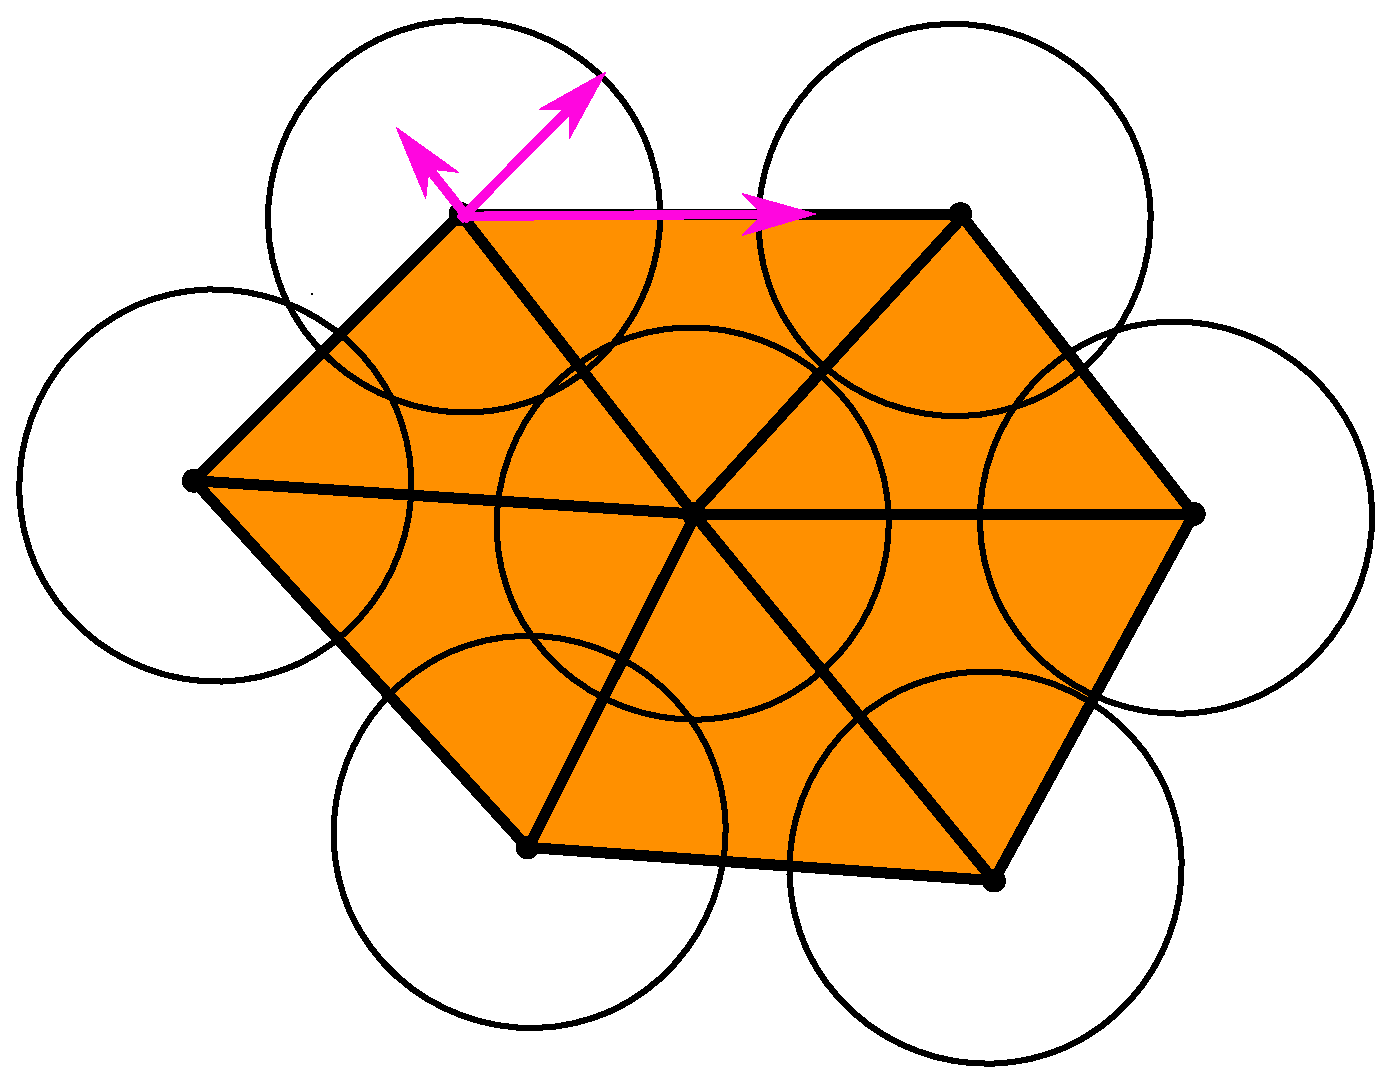
\includegraphics[width=\textwidth]{bilder/meshCorrector/EdgeLaw.eps}
      \caption[Kantenkräfte für optimale Kantenlängen]{Kantenkräfte für an einem Knoten \( k = 1 \). Die eingezeichneten Radii entsprechen \( \frac{l^{*}}{2} \).}
      \label{edgeLaw}
      \end{minipage}
      \hfill
      \begin{minipage}[t]{0.45\textwidth}
      \raisebox{10pt}{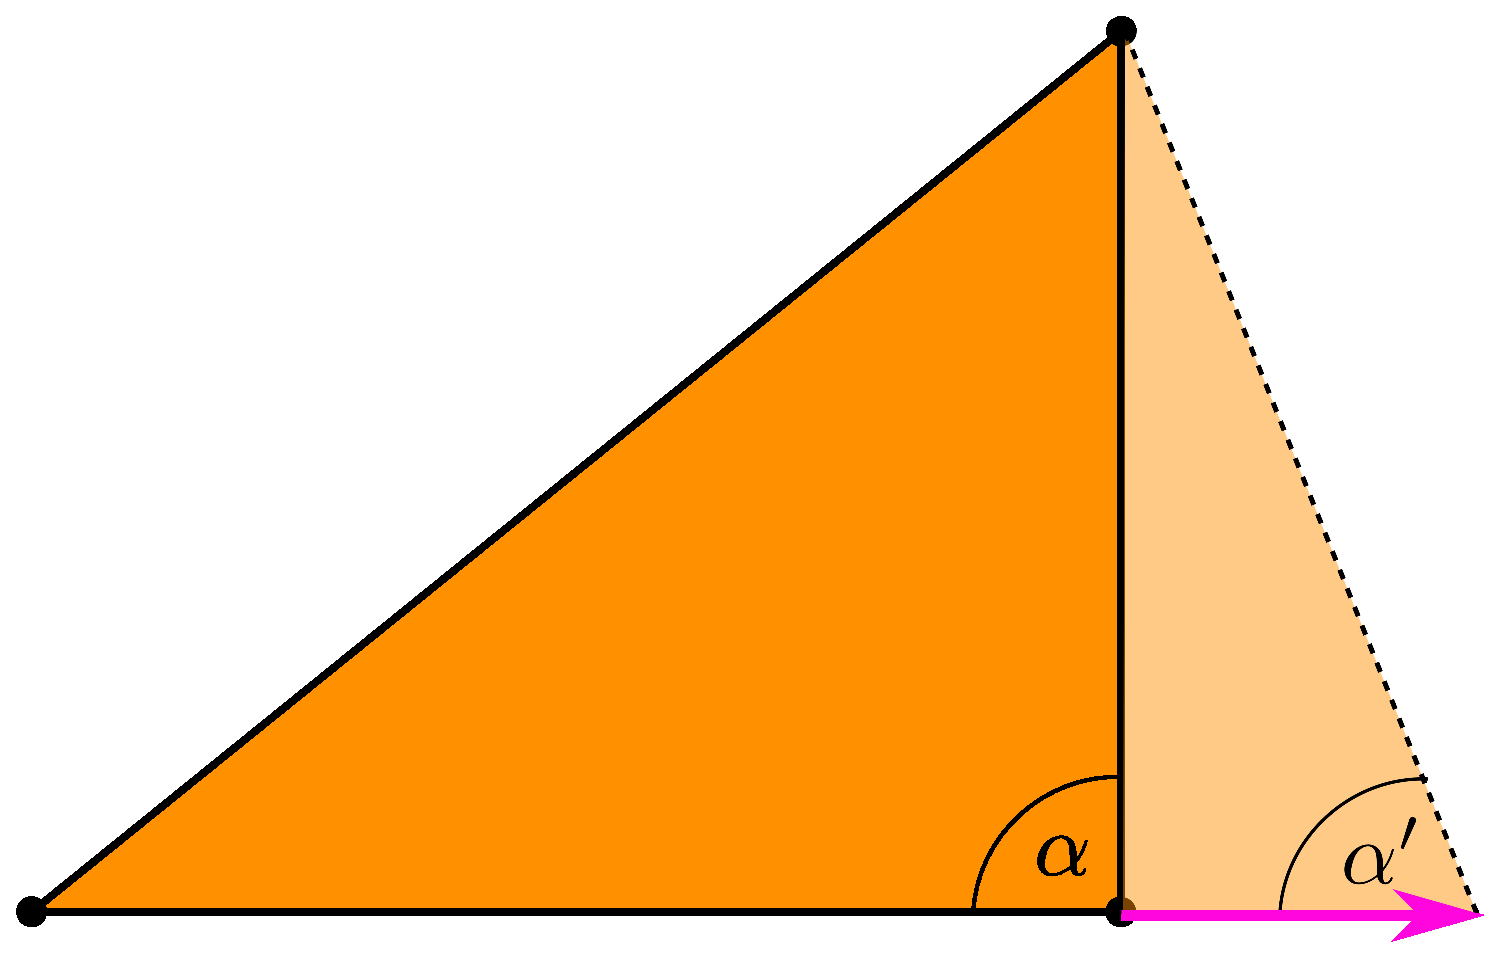
\includegraphics[width=\textwidth]{bilder/meshCorrector/AngleLaw.eps}}
      \caption[Winkeländerung durch Verschiebung]{Eine Verschiebung des Knotens entlang einer Kante verändert den Winkel.}
      \label{angleLaw}
      \end{minipage}
    \end{figure}

  \subsubsection{Optimale Winkel}
    Ein weiterer heuristischer Ansatz bezieht sich direkt auf die inneren Winkel eines Dreieckelements. 
    Wie in Abbildung \ref{angleLaw} angedeutet bewirkt eine Verschiebung entlang der Kante eine änderung des Winkels.
    Wird dabei, wie in Abbildung \ref{angleLaw}, die Kante länger, dann wird der Winkel an dem zuverscheibenen Knoten kleiner, et vice versa. 
    \begin{align}
       F^{A}_{\sigma^{0}\prec\sigma^{1}_{i}\prec\sigma^{2}} &:= \cos\measuredangle(\vec{e}_{0},\vec{e}_{1}) - c \label{angleForce}\\
                              &= \frac{\vec{e}_{0} \cdot \vec{e}_{1}}{\|\vec{e}_{0}\|\|\vec{e}_{1}\|} - c \\
       \vec{e}_{i} := \vec{e}_{\sigma^{1}_{i}} &= \vec{x}_{v_{i}} - \vec{x}_{\sigma^{0}}\\
    \end{align}
    mit \( i\in\{0,1\} \) und \( c\in[-1,1] \). 
    \( v_{i} \) ist also der Knoten, der mit \( \sigma^{0} \) die gemeinsame Kante \( \sigma^{1}_{i} \) 
    im Dreieck \( \sigma^{2} = [\sigma^{0},v_{0},v_{1}] \) hat.
    
    Eine sinnvolle Wahl für die Konstante ist \( c = \cos \frac{\pi}{3} = 0.5\).
    Sie würde in einer flachen Triangulation mit hexagonaler Struktur bewirken, dass sich keine Kräfte entwickeln, falls alle Dreiecke bis auf Rotation und Translation gleich sind.

  \subsubsection{Kombination der Kantenkräfte}
    Es hat sich gezeigt, dass \eqref{edgeForce} und \eqref{angleForce} gerade auf komplizierteren Gebieten einzeln entweder nicht das gewünschste Resultat liefern oder insatbil sind.
    Deshalb kombinieren wir die beiden Kräfte linear:
    \begin{align}
      F^{\text{Gesamt}}_{\sigma^{0}\prec\sigma^{1}} &:= D \cdot F^{L}_{\sigma^{0}\prec\sigma^{1}} + (1-D) \cdot F^{A}_{\sigma^{0}\prec\sigma^{1}}
    \end{align}
    mit \( D\in[0,1] \).
    Algorithmus \ref{AlgoForces} zeigt wie die resultierenden Kräfte auf einem Dreieckelement berechnet werden können. 
    Um alle Knotenkräfte\footnote{d.h. \((\vec{F}_{i})_{i=1,\ldots, N_{\sigma^{0}}}\in (\R^{3})^{N_{\sigma^{0}}} \)} zu erhalten müssen wir nur noch diese Element-Knotenkräfte aufassemblieren. 
    
  \subsubsection{Projektion der Kraftvektoren}
    Des Weiteren, wie im Algorithmus \ref{AlgoForces} zu sehen, wird der Kraftvektor \( \vec{F}_{i} \) in den Tangentialraum projeziert, das heißt
    \begin{align}
      \vec{F}_{T_{p}M,i} = \vec{F}_{i} - (\vec{F}_{i}\cdot\vec{\nu_{i}})\vec{\nu_{i}}
    \end{align}
    wobei der Normalenvektor \( \vec{\nu_{i}}  \) am Knoten \( \sigma^{0}_{i} \) entweder als bekannt vorrausgesetzt ist,
    über eine signierte Distanze Funktion \( \varphi \) ermittelt wird, also
    \begin{align}
      \vec{\nu_{i}} = \frac{\nabla\varphi}{\|\nabla\varphi\|}(\vec{x}_{i})
    \end{align}
    oder über die Elementnormalen approximiert wird
    \begin{align}
      \vec{\nu_{i}} = \frac{1}{|\circlearrowleft\sigma^{0}_{i}|} \sum_{\sigma^{2}\succ\sigma^{0}_{i}} |\sigma^{2}|\cdot \vec{\nu}_{\sigma^{2}}
    \end{align}
    Somit kann im expliziten Eulervefahren \eqref{euler} \( \vec{F}_{T_{p}M,i}\) statt \( \vec{F}_{i} \) verwendet werden.
    Das müssen wir nicht machen, aber es bringt Vorteile. 
    Zum einen könnten Knoten soweit in Normalenrichtung verschoben werden, dass die nachfolgende Projektion den Knoten falsch abbildet und das Gitter zerstört wird 
    (vgl. Abb. \ref{AbbFatalEuler}), zum anderen wird die Projektion in \eqref{euler} oft iterativ gelöst (vgl. \ref{SubSubSecPhiProject}) und je weiter weg wir den Knoten von der
    Mannigfaltigkeit verschieben um so schlechter ist die Startnährung für das iterative Verfahren.
    \begin{figure}
      \centering
      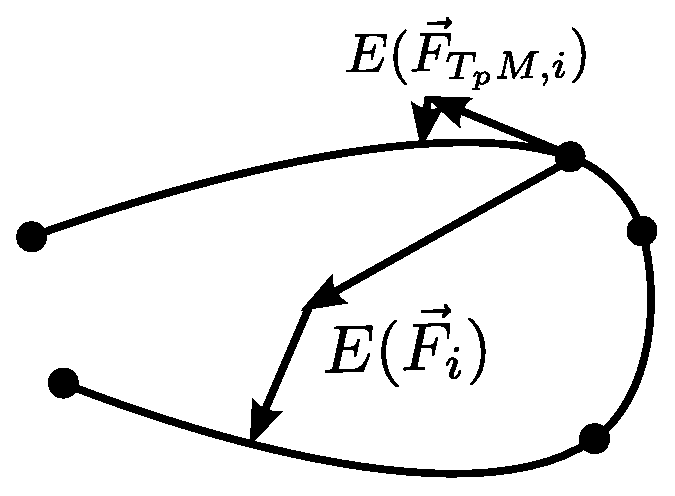
\includegraphics[width=0.5\textwidth]{bilder/meshCorrector/fatalEuler.eps}
      \caption[Euler mit und ohne Vorprojektion]{Eindimensionales Extrembeispiel für ein Schritt Euler-Explizit \( E \) (inkl. Nachprojektion \( \pi \))
                                                  eines Knotens mit und ohne Vorprojektion des Kraftvektors \( \vec{F}_{i} \)
                                                 zu \( \vec{F}_{T_{p}M,i}\). 
                                                 Ohne Vorprojektion kann es zu einem unzulässigen Gitter kommen.}
      \label{AbbFatalEuler}
    \end{figure}


  % start merge
  
  \subsection{Beispiele}
    
    \subsubsection{Ellipsoid}
      Wir wollen nun ein geeignetes Gitter für ein Ellipsoid erstellen (vgl. Appendix \ref{heineC}).
      Zur Verfügung steht uns eine Starttriangulierung der Einheitssphäre mit zirka 1000 Knoten.
      Es ist fast überall eine hexagonale Struktur vorhanden bis auf 12 Defekte, genauer, an 12 Knoten
      befinden sich pentagonale 1-Ringe. 
      Dieses Startgitter wird nun auf den Ellipsoid projeziert (vgl. \ref{SubSubSecPhiProject}).
      Wie in Abbildung \ref{AbbEllipsoid} zu sehen, ist ein wohlzentrierter Simplizialkomplexe nach nur
      wenigen Eulerschritten \eqref{euler} erreicht. 
      Der größte Winkel nimmt aber weiterhin logarithmisch ab. 
      Nach zirka 200 Schritten hat er sein Minimum erreicht und steigt danach wieder leicht.
      Das ist nicht verwunderlich, denn kleinere Winkel sind nicht das einzige Optimalitätskriterium.
      Geplottet wurde auch das Integralmittel der größten Winkel der Dreiecke, das heißt
      \begin{align}
         \alpha_{max} = blub
      \end{align}

      
      \begin{figure}
        \begin{minipage}[t]{0.45\textwidth}
        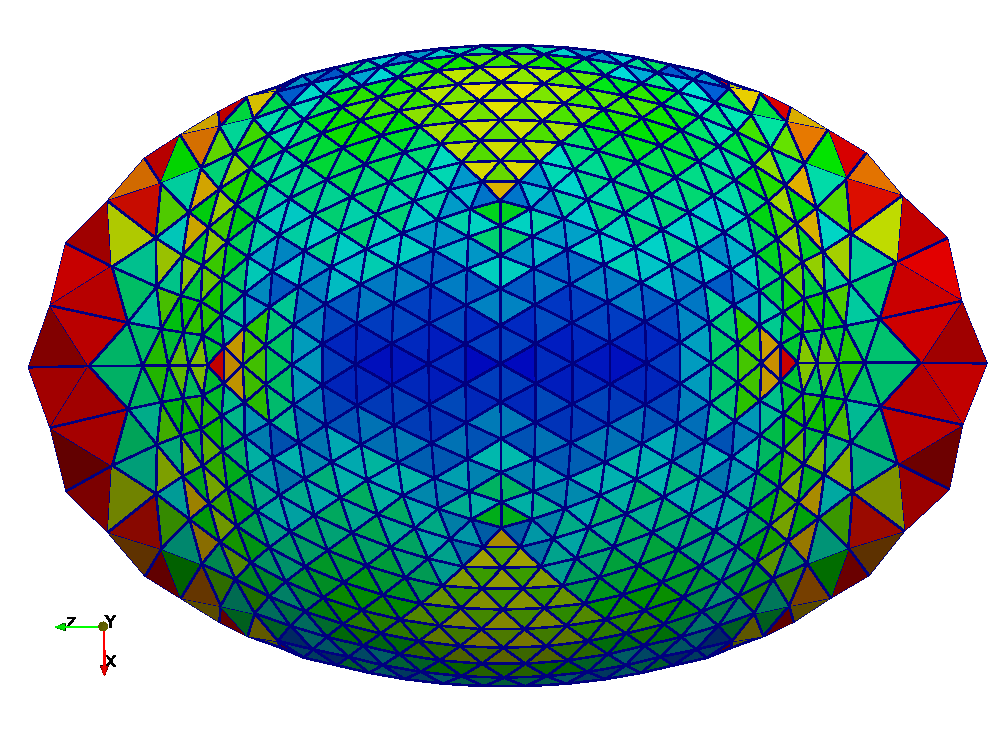
\includegraphics[width=\textwidth]{bilder/meshCorrector/Before_AnglesHeine51c_1k_h001_k10_c07.eps}
        \end{minipage}
        \hfill
        \begin{minipage}[t]{0.49\textwidth}
        {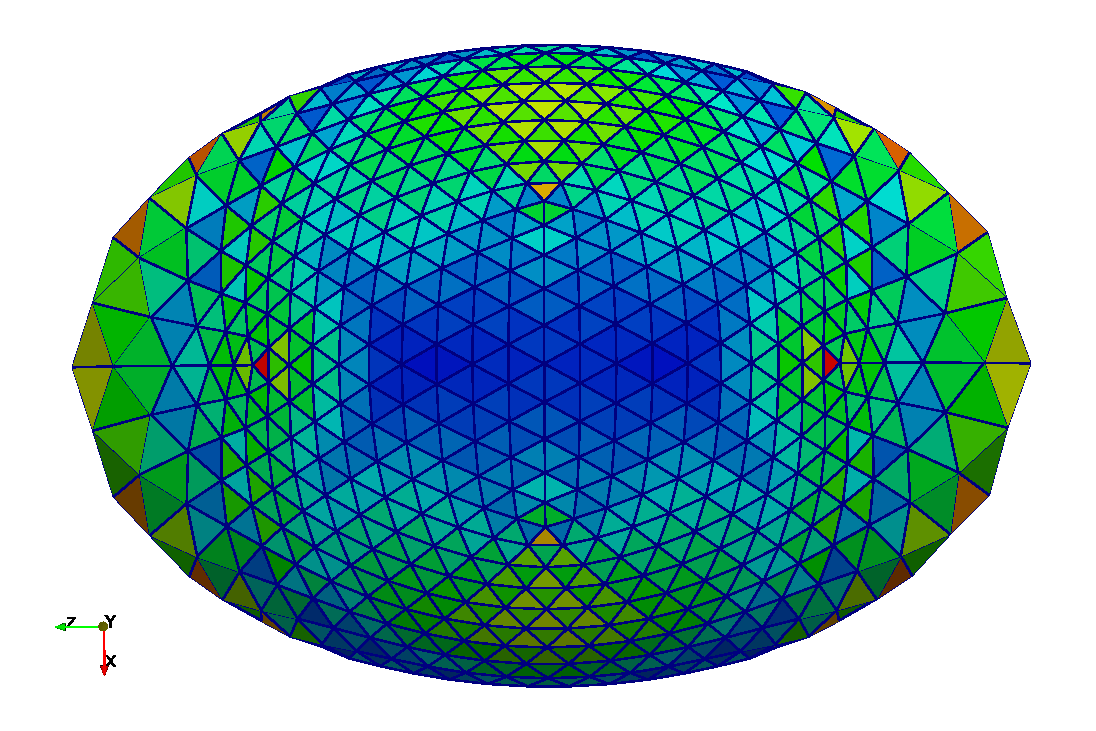
\includegraphics[width=\textwidth]{bilder/meshCorrector/step7_AnglesHeine51c_1k_h001_k10_c07.eps}}
        \end{minipage}
        \begin{minipage}[t]{0.49\textwidth}
        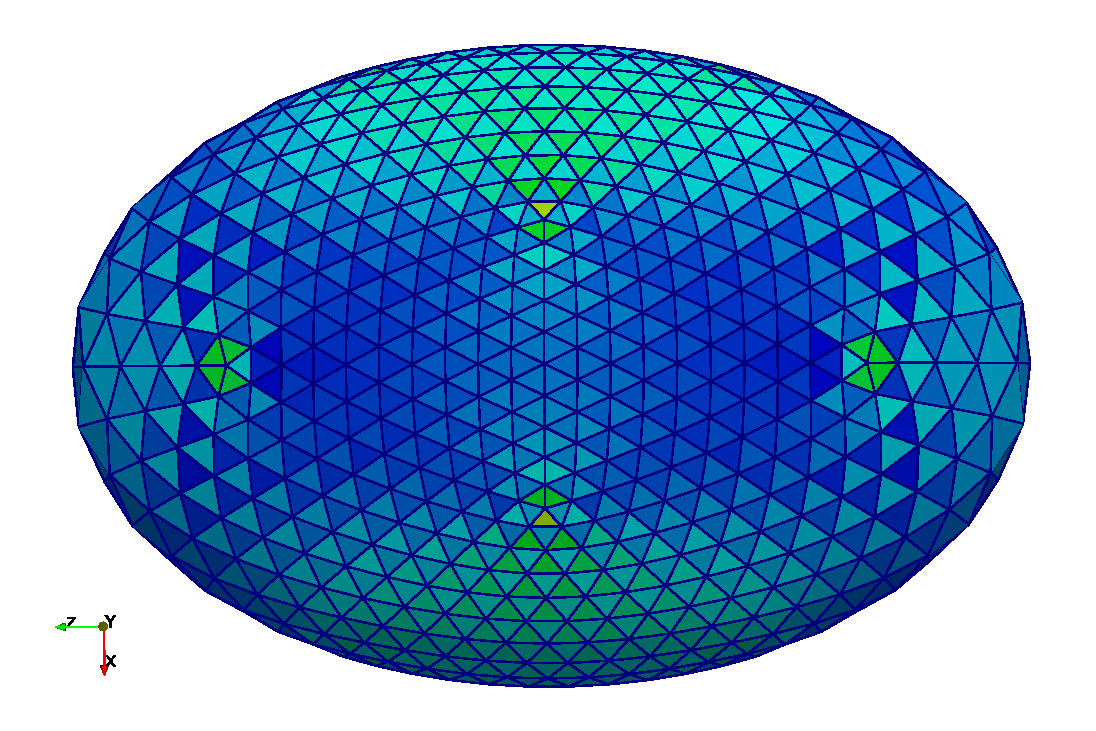
\includegraphics[width=\textwidth]{bilder/meshCorrector/step1000_AnglesHeine51c_1k_h001_k10_c07.eps}
        \end{minipage}
        \hfill
        \begin{minipage}[t]{0.5\textwidth}
        {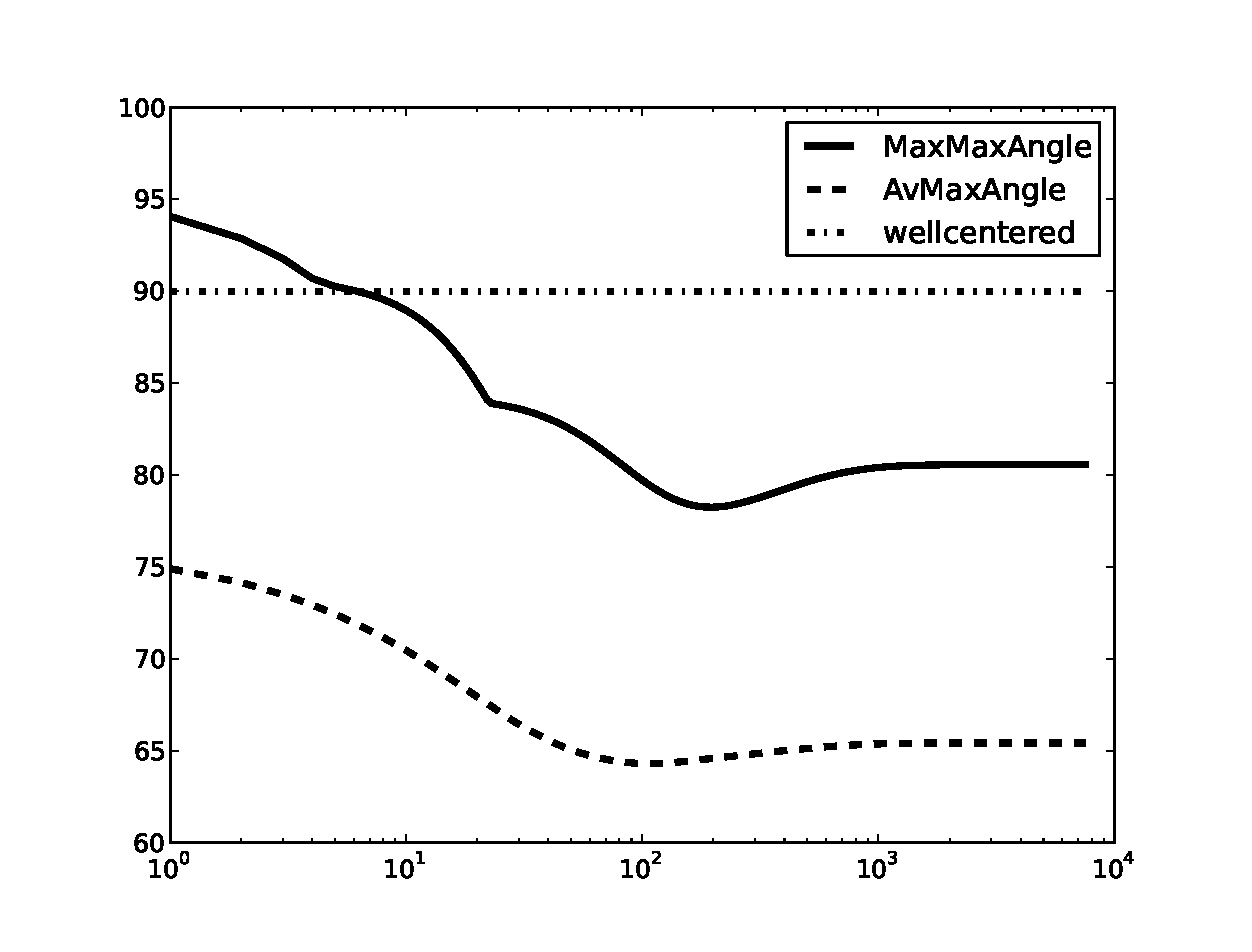
\includegraphics[width=\textwidth]{bilder/meshCorrector/step7500_AnglesHeine51c_1k_h001_k10_c07.eps}}
        \end{minipage}
        \begin{minipage}[t]{\textwidth}
        {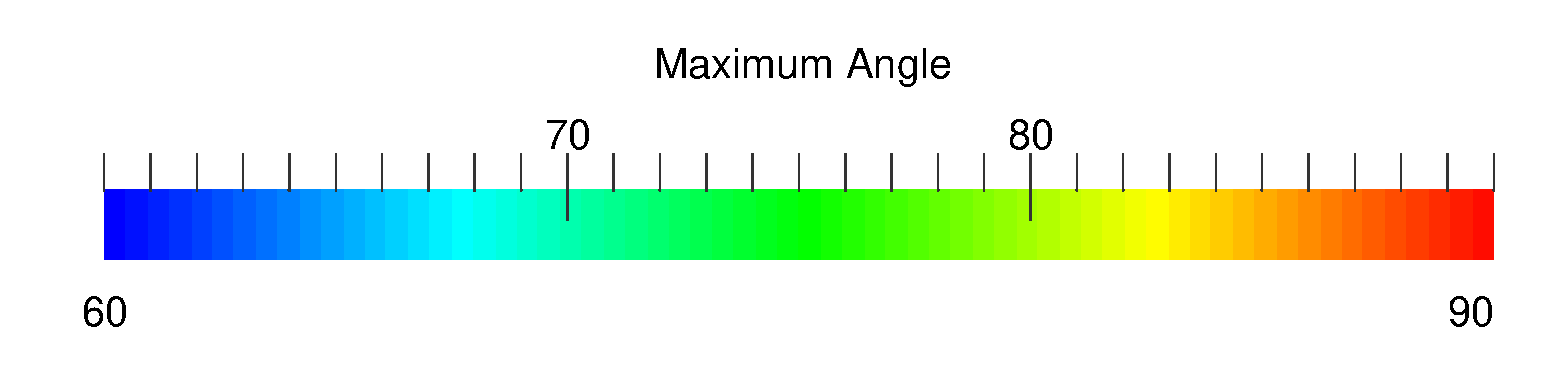
\includegraphics[width=\textwidth]{bilder/meshCorrector/Angle6090_scaleBar.eps}}
        \end{minipage}
        \caption[Gittergenerierung: Ellipsoid]
                {Parameter: h = 0.01; k = 1; c = 0.7. 
                 Von links oben nach rechts unten: 
                 Startgitter (keine Wohlzentriertheit, maximaler Winkel ca. \ang{95.9}); 
                 nach 7 Eulerschritten (Wohlzentriertheit);
                 nach 1000 Eulerschritten (danach keine signifikanten Veränderungen mehr);
                 (semilog)Eulerschritte-Winkel-Plot (Maximum und Integralmittel)}
         \label{AbbEllipsoid}
      \end{figure}

  % end merge

  \section{Implizit gegebene Oberflächen}
    Oftmals ist eine Oberfläche \( M\subset\R^{3} \) nicht explizit über eine Immersion 
    \begin{align}
      X:(u,v)\mapsto X(u,v)\in\R^{3}
    \end{align}
    gegeben, sondern über den 0-Level-Set einer signierten Distanzfunktion
    \begin{align}
      \varphi = \pm\text{dist}(\cdot,M) = \pm\inf_{\vec{x}\in M} d(\cdot,\vec{x})
    \end{align}
    mit einer beliebigen (ausreichend glatten) Metrik \( d \) im \( \R^{3} \).
    Die 2-Mannigfaltigkeit ist dann definiert durch 
    \begin{align}
      M = \left\{ \vec{x}\in\R^{3} \middle| \varphi(\vec{x})=0 \right\} \text{.}
    \end{align}
    Solche implizit beschriebenen Oberflächen liegen zum Beispiel bei 3D-Phasenfeldproblemen vor 
    (z.B. Allen-Cahn-, Cahn-Hilliard- oder Phase-Field-Crystal-Modell). 
    Die Distanzfunktion\footnote{auch Phasen- oder Ordnungsfunktion genannt} \( \varphi:\R^{3}\rightarrow\R \) ist dort gerade die Lösung dieser Probleme
    und das 0-Niveau dieser Funktion beschreibt die Phasengrenzen.

    Wir treffen hier die Konvention, dass "`außen"' \( \varphi > 0 \) gilt und "`innen"' \( \varphi < 0 \).
    Dadurch zeigt der Gradient \( \nabla\varphi(\vec{x}) \) für alle \( \vec{x}\in M \) in Richtung der äußeren Normalen.
    "`Außen"' und "`innen"' ist durch die Orientierung der Mannnigfaltigkeit gegeben. 
    In Falle von 2-Mannigfaltigkeiten ohne Rand, ist "`innen"' gerade das von der Oberfläche umschlossene Gebiet im \( \R^{3} \).

    \subsection{Numerische Projektion}
      Wenn bei einem Simplizialkomplex, welches die Oberfläche approximiert, neue Knoten enstehen oder vorhandene verschoben werden sollen,
      dann ist es notwendig diese Knoten auf die Mannigfaltigkeit zu projezieren. 
      Denn eine Bedingung an den Simplizialkomplex ist, dass die Knoten dort und auf dem abstrakten Simplizialkomplex übereinstimmen.

      Gesucht ist also das
      \begin{align}
        \argmin_{\vec{x}\in M} \|\vec{y} - \vec{x}\|
      \end{align}
      für den Knoten mit den Koordinaten \( \vec{y} \), der sich noch nicht auf der Mannigfaltigkeit \( M \) befindet 
      und damit \( \varphi(\vec{y}) \neq 0 \) gilt.

      

  \begin{fazit}
  dfsd
  \end{fazit}
